\documentclass{article}
\usepackage{graphicx}
\usepackage{titling}  % For custom title page
\usepackage{circuitikz}
\usepackage{amsmath}
\usepackage{amssymb}
\usepackage{booktabs,tabu}


\title{Experiment 1: Basic Filter Design}
\author{Samyak Sheersh, Aryam Shankar}
\date{06 August 2024}
\newcommand{\subtitle}[1]{%
  \posttitle{%
    \par\end{center}
    \begin{center}\large#1\end{center}
    \vskip0.5em}%
}

\begin{document}

% Custom title page
\begin{titlepage}
    \centering
    
\includegraphics[width=0.2\textwidth]{KGP_logo.png}\par\vspace{1cm}
    {\scshape\LARGE Department of Electronics and Electrical Communication Engineering, IIT Kharagpur\par}
    \vspace{1cm}
    {\huge\bfseries Experiment 1: Sampling\par}
    \vspace{1.5cm}
    {\Large\itshape Samyak Sheersh, Anubhav Mitra\par}
    \vfill
    % Identifying information at the bottom
    {\large Roll Numbers: 22EC30045, 22EC30007\par}
    {\large Group Number: 24\par}
    \vfill
    {\large 07 August 2024\par}
\end{titlepage}

\section{Tasks}
\subsection{Sampling of a sinusoidal waveform}
\begin{enumerate}
  \item Take an analog waveform:
    $$
    x(t)=10\cos(2\pi\times 10^3t)+6\cos(2\pi\times2\times10^3t)+2\cos(2\pi\times4\times10^3t)
    $$
  \item Sample if at $F_s=12kHz$
  \item Obtain DFT of $x(t)$ with N=$\{64,128,256\}$ points and plot the respective magnitude spectra.
  \emph{Note the change in spectrum as N is increased}
\end{enumerate}

\subsection{Sampling at below Nyquist rate and effect of aliasing}
\begin{enumerate}
  \item Repeat above with $F_s= \{8kHz, 5kHz, 4kHz\}$
  \item Find out from the spectrum, what are the aliases of the original frequencies present in $x(t)$ when the sampling rate is below the Nyquist rate.
\end{enumerate}

\subsection{Spectrum of a square wave}
\begin{enumerate}
  \item Take a square wave with time period T = 1ms(F=1kHz)
  \item Sample it at F=20kHz
  \item Obtain DFT of the sampled square wave with N=256 and plot the result
\end{enumerate}

\subsection{Interpolation or upsampling}
\begin{enumerate}
  \item Take a lowpass signal of bandwidth 6kHz
  \item Sample it at $F_{s1}=12kHz$
  \item Insert a zero between every two samples
  \item Pass it through a lowpass filter of cutoff frequency 6kHz
    \emph{Note that at step 4, the LPF is a digital filter, and sampling frequency to be used is $F_{s2}=24kHz$}
  \item Plot the output of the lowpass filter and compare it with the original signal sampled at $F_s=24kHz$
    \emph{It may differ by a delay and a scaling factor}
\end{enumerate}
\newpage
\section{Graphs and Diagrams}
\subsection{Task 1.1}
\begin{figure}[!ht]
    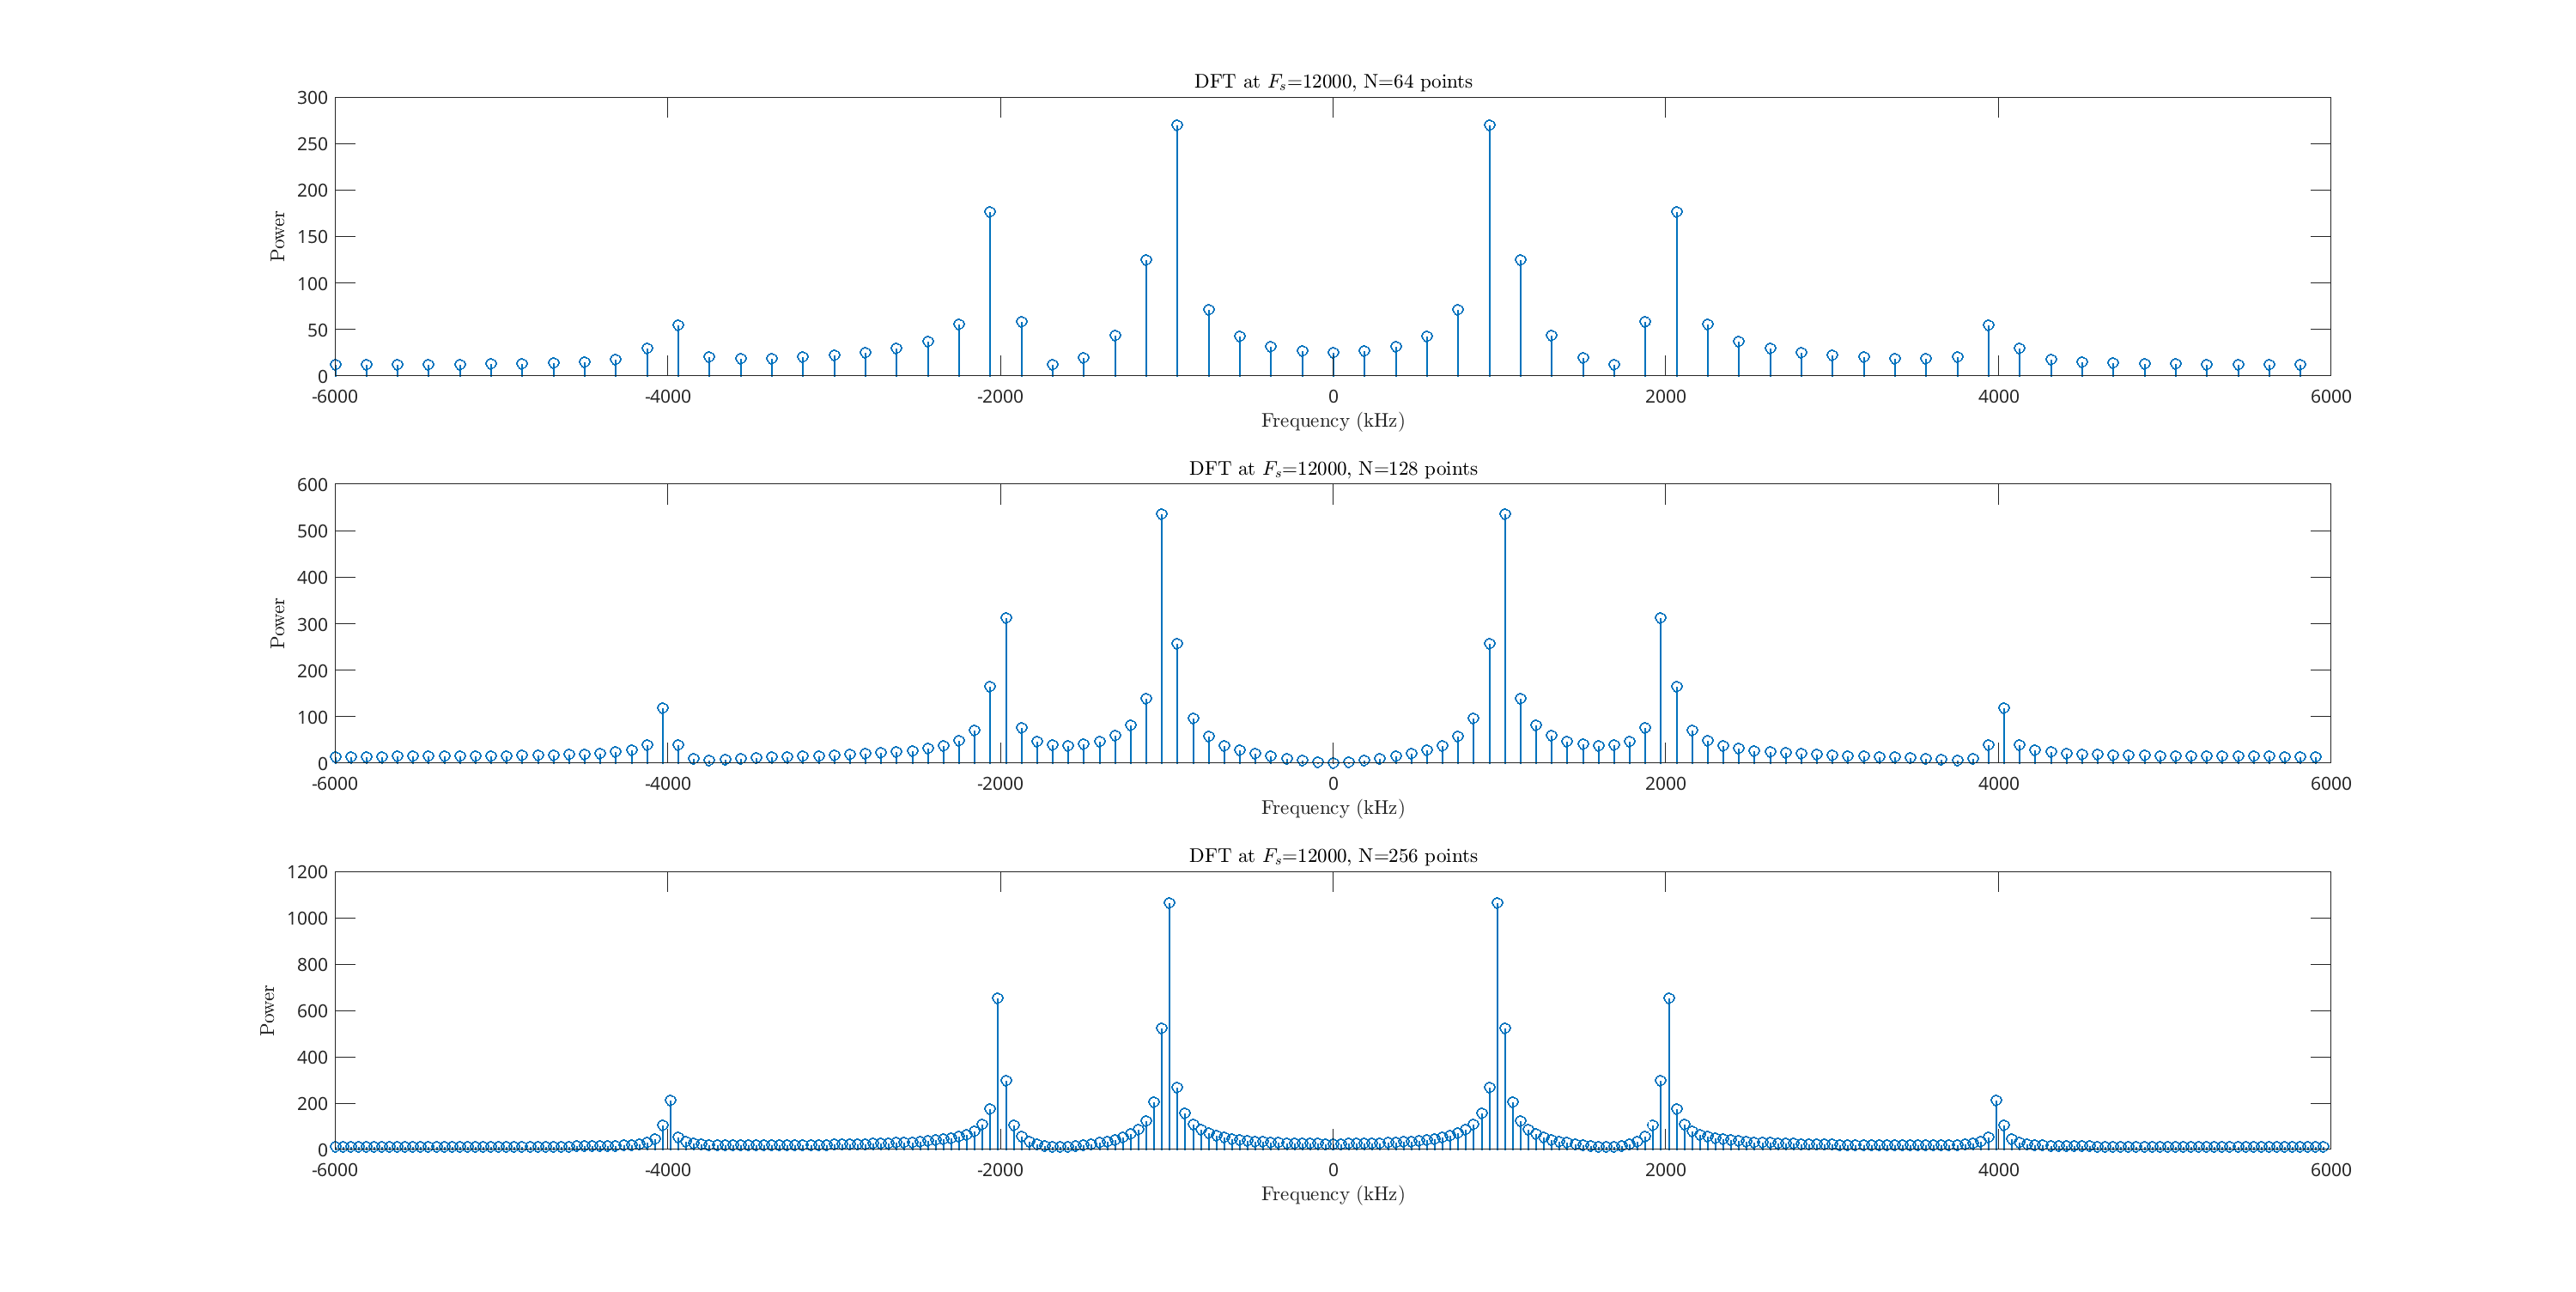
\includegraphics[width=\textwidth]{Ass1a.png}
\end{figure}
\newpage
\subsection{Task 1.2}
\begin{figure}[!ht]
    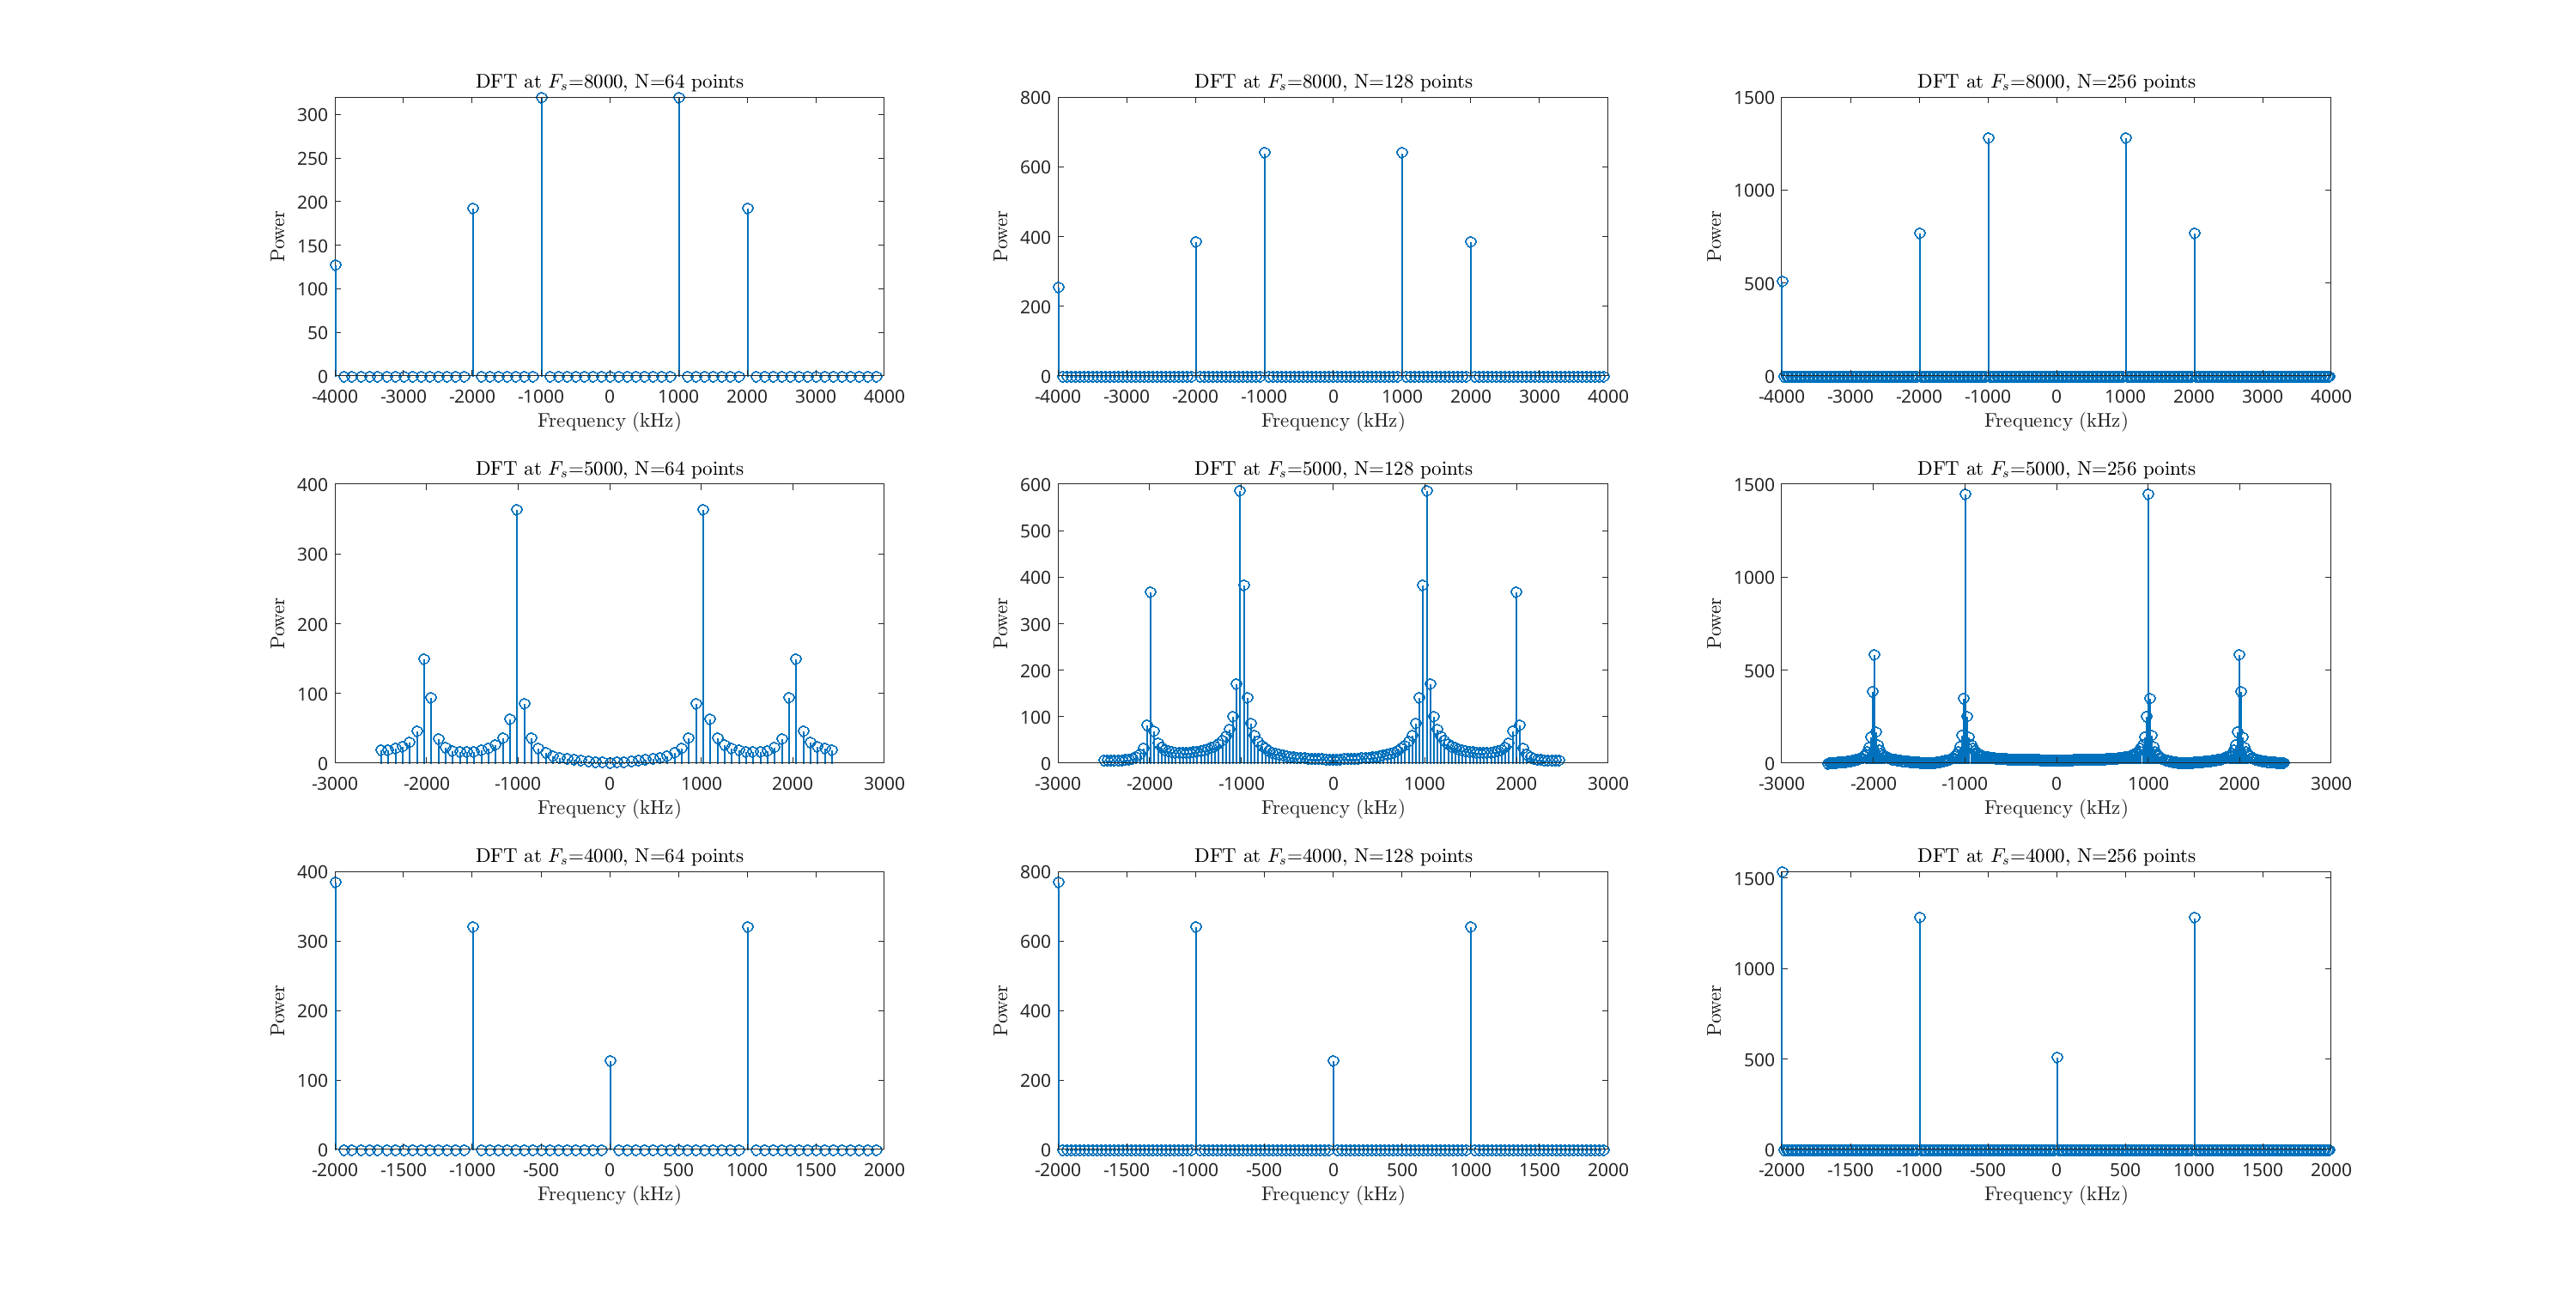
\includegraphics[width=\textwidth]{Ass1b.png}
\end{figure}
\subsection{Task 1.3}
\begin{figure}[!ht]
    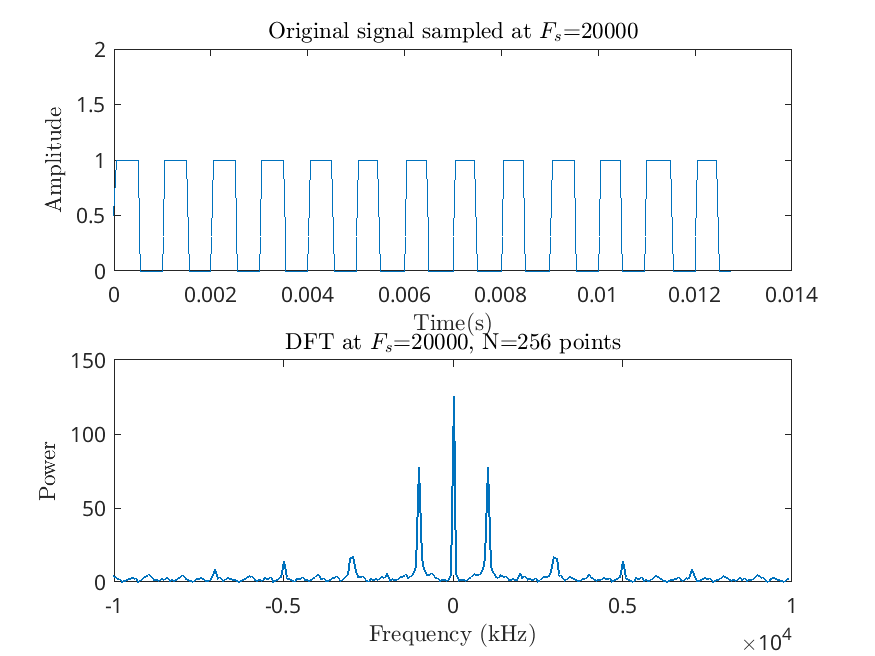
\includegraphics[width=\textwidth]{Ass1c.png}
\end{figure}

\subsection{Task 1.4}
\begin{figure}[!ht]
    \caption{The input signal}
    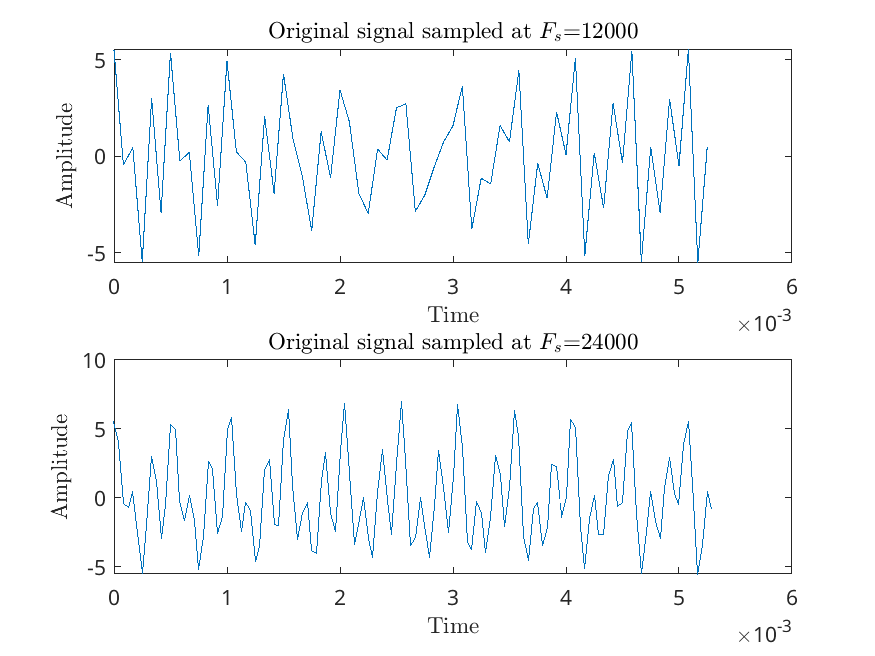
\includegraphics[width=\textwidth]{Ass1da.png}
\end{figure}

\begin{figure}[!ht]
    \caption{The upsampled and filtered signals}
    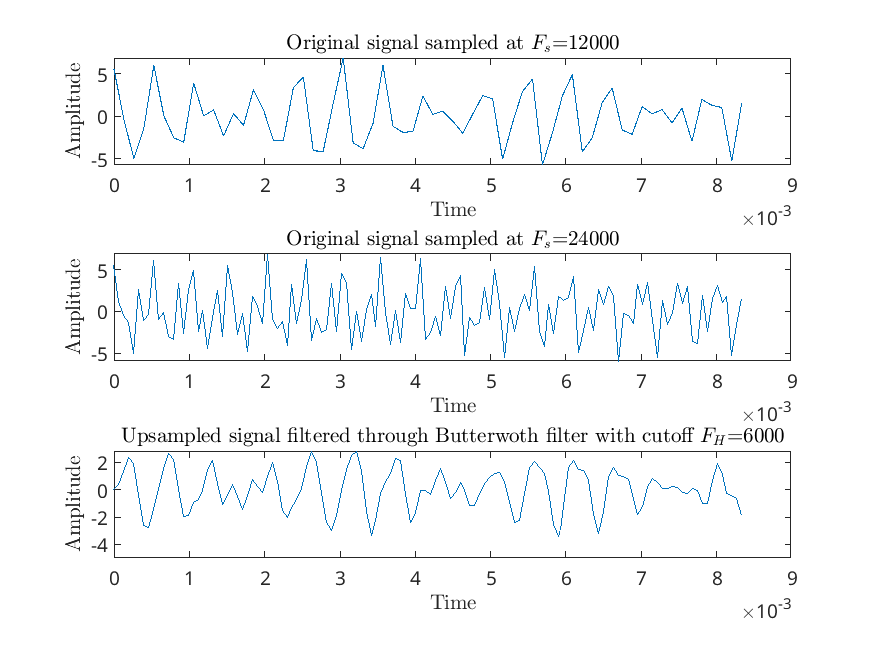
\includegraphics[width=\textwidth]{Ass1db.png}
\end{figure}

\newpage

\section{Discussions}
\subsection{Samyak Sheersh}
\begin{enumerate}
  \item In part 1.1, we sampled at a rate above the Nyquist rate and in every plot, we see some sharp peaks, which correspond to the composite frequencies present in the original signal. However, as we increase the number of samples, we see the peaks grow sharper and the values in the middle shrink down. This is reflective of the fact that a larger sample size will better approximate the continuous Fourier transform which will just have $\delta$'s of different strength on the frequencies in the signal

  \item In part 1.2, as we repeat the plots for lower sampling frequencies, the variation of N provides similar results as 1.1.We, howeverm observe aliasing for sampling below the Nyquist rate. 
    \begin{itemize}
      \item For sampling exactly at 8kHz, we find that the peak at 4kHz gets omitted, however we still observe a peak at $-$4kHz.

      \item For a sampling rate of 5kHz, we observe additional peaks at 1kHz and 2kHz due to aliasing as these are further multiples of the 4kHz component of the original signal modulo 5. 

      \item For sampling at 4kHz, we observe a peak at 0Hz, inferring a DC value which occurs due to the overlap of the 4kHz components as their multiples modulo 4 give zero and the sampling rate is lower than their Nyquist rate. Just like the first case where we saw -4kHz but not +4kHz, we see that we also get a peak at -2kHz but not at +2kHz
  \end{itemize}

  \item In part 1.3, we see that the pulse signal is not a continuous signal and has jumps each time it flips between 0 and 1. Thus it can never be truly approximated and Gibbs phenomena will occur around the discontinous. Since we are also limiting the bandwidth to the 10th harmonic at 20 kHz, we'll not get the full range of frequencies. 

  \item In part 1.4, we observe that the filtered signal is delayed and has half the amplitude of the original signal. Also compared to the signal sampled at double the original frequency, we clearly see that the higher frequencies have been filtered out and as a result the signal is much smoother. We believe that because of upsampling, the sharp changes coming due to the fact that it was going back to zero were interpreted as high frequency and thus filtered off.  
\end{enumerate}



\end{document}
